\documentclass[xetex,mathserif,serif]{beamer}
\usepackage{polyglossia}
\setdefaultlanguage[babelshorthands=true]{russian}
\usepackage{minted}
\usepackage{tabu}

\useoutertheme{infolines}

\usepackage{fontspec}
\setmainfont{FreeSans}
\newfontfamily{\russianfonttt}{FreeSans}

\definecolor{links}{HTML}{2A1B81}
\hypersetup{colorlinks,linkcolor=,urlcolor=links}

\setbeamertemplate{blocks}[rounded][shadow=false]
\setbeamercolor*{block title alerted}{fg=red!50!black,bg=red!20}
\setbeamercolor*{block body alerted}{fg=black,bg=red!10}

\tabulinesep=0.8mm

\title{О курсовых}
\author{Юрий Литвинов}
\date{08.05.2018г}

\begin{document}

	\frame{\titlepage}

	\begin{frame}
		\frametitle{Про тексты курсовых}
		\framesubtitle{Структура отчёта}
		\begin{itemize}
			\item Титульный лист (\url{http://math.spbu.ru/rus/study/alumni\_info.html})
			\item Оглавление
			\item Введение в предметную область, постановка задачи
			\item Обзор литературы и существующих решений
			\item Описание предлагаемого решения, сравнение с существующими
			\item Заключение
			\item Список источников (ГОСТ Р 7.0.5--2008)
			\item Приложения (если есть)
		\end{itemize}
	\end{frame}

	\begin{frame}
		\frametitle{Введение}
		\begin{columns}
			\begin{column}{0.6\textwidth}
				\begin{itemize}
					\item Известная информация, ``Background''
					\item Неизвестная информация, ``Gap''
					\begin{itemize}
						\item Актуальность темы
						\item Практическая значимость
					\end{itemize}
					\item Цель работы, ``Гипотеза'' 
					\item Задачи, необходимые для достижения цели, ``Подход''
				\end{itemize}
			\end{column}
			\begin{column}{0.4\textwidth}
				\begin{center}
					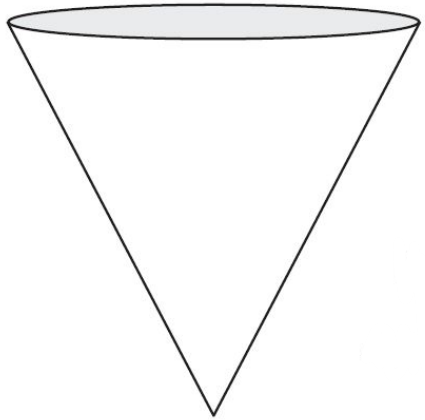
\includegraphics[width=\textwidth]{introductionCone.png}
				\end{center}
			\end{column}
		\end{columns}
	\end{frame}

	\begin{frame}
		\frametitle{Обзор}
		\begin{itemize}
			\item Обзор существующих решений
			\begin{itemize}
				\item Цель и фокус обзора
				\item Критерии сравнения
				\item Выводы
			\end{itemize}
			\item Обзор используемых чужих результатов
			\begin{itemize}
				\item  Всё, написанное и придуманное не вами --- в обзор
			\end{itemize}
			\item Должен соотноситься с темой и с фокусом работы
		\end{itemize}
	\end{frame}

	\begin{frame}
		\frametitle{Описание решения}
		\begin{itemize}
			\item Желательно, чтобы разделы отвечали решению задачи из списка задач во введении
			\item Аргументированное обоснование принятых решений и отказа от альтернатив
			\item Описание программной реализации, архитектура
			\item Эксперименты и апробация
			\item Выводы и обсуждение
		\end{itemize}
	\end{frame}

	\begin{frame}
		\frametitle{Заключение}
		\begin{itemize}
			\item Перечисление результатов, выносимых на защиту
			\item Должно быть согласовано с постановкой задачи (вплоть до полного её повторения)
			\item Должно быть согласовано с текстом
			\item Никаких результатов из ниоткуда
		\end{itemize}
	\end{frame}

	\begin{frame}
		\frametitle{Общие замечания}
		\begin{itemize}
			\item Каждый рисунок --- пронумерован и подписан, есть ссылка из текста
			\item На каждый элемент списка литературы ссылка из текста
			\item Никакого плагиата!
			\item Полезно сначала написать план
			\item \url{https://papeeria.com/}
		\end{itemize}
	\end{frame}

\end{document}
